\documentclass[12pt]{article}
\usepackage{fullpage}
%\usepackage{fancyhdr}
\usepackage{color}
\usepackage{pdfpages}
\usepackage{hyperref}

\hypersetup{
	colorlinks=true,
	linkcolor=black,
	filecolor=magenta,      
	urlcolor=blue,
}

%\pagestyle{fancy}

\begin{document}
	\begin{titlepage}
	\begin{center}
		
	
	\vspace*{1in}
	{\Huge \textbf{FRC Advanced Control System Development: Part IV}}\\
	\vspace{0.25in}
	{\LARGE Robot Command \& Telemetry with Ball COSMOS}\\
	\vspace{0.5in}
	{\Large Carlos Gross Jones}\\
	\vspace{0.1in}
	{\Large FRC Team 696}\\
	\vspace{0.1in}
	{\Large \today}\\
\end{center}
	
\end{titlepage}


\section{Introduction}
\par This paper will cover a method of capturing CAN traffic on the RoboRIO, as well as encapsulating the CAN frames using the CCSDS Space Packet Protocol and transmitting them over the robot network. Later papers in this series will address how to capture, analyze, visualize, and log the resulting data streams. 


\section{Monitoring CAN Traffic}
\par Since so much of the communication on the robot occurs over the CAN bus (all PDP voltage/current telemetry, PCM status and commands, smart motor controller data, etc.), being able to monitor and process CAN frames immediately provides a wealth of telemetry and diagnostic information. A basic way of doing this is to simply use a device API to read the CAN data of interest, and then relay that data to a remote machine, using for example NetworkTables. However, this technique has several limitations. First, the telemetry is restricted to that data which can be accessed through existing API calls. Second, adding statements to poll effectively all APIs for all devices in use, and then publish that data, results in a tremendous amount of code cluttering up the user program. Finally, since a certain amount of decoding would have to be done by the RoboRIO, this would steal precious CPU cycles. 

\par Therefore, it is preferable to relay raw CAN frames to a remote machine, and process them on a more capable platform. There are several ways to do this. One would be to use some kind of CAN bridge physically connected to the bus, and to a data channel to the remote machine. The \href{https://copperhilltech.com/pican-2-can-interface-for-raspberry-pi-2-3/}{PiCAN2} and \href{https://www.microchip.com/DevelopmentTools/ProductDetails/PartNO/APGDT002}{Microchip CAN Bus Analyzer Tool} come to mind. However, since the RoboRIO already has a built-in CAN interface, as well as an Ethernet connection, it seems preferable to stream CAN frames from the RoboRIO, over Ethernet, across the WiFi link, to a telemetry computer. This allows realtime monitoring of all data that transits the CAN bus, in realtime, with minimal burden to the RoboRIO. 

\par First, a brief overview of the RoboRIO/Athena/WPIlib CAN stack is in order. The actual CAN interface on the RoboRIO PCBA is routed to the Zynq Z-7020 processor\footnote{I don't know if the CAN interface is routed directly to the ARM core, or if it goes through the FPGA.}. Linux instantiates the CAN port as character device \texttt{/dev/ni/niembcanzynqk:0\textbackslash niembcan\_ucan\textbackslash 0}. This device is accessed exclusively by \texttt{/usr/local/frc/bin/FRC\_NetCommDaemon},  commonly known as FRCNetComm. This binary, as far as I can tell, is a black box; only the header is publicly available. User software then interacts with the FRCNetComm interface (either directly or via JNI). More specifically, CAN traffic is handled with the CANSessionMux framework. This allows multiple processes to send and receive packets through a single physical interface. WPIlib provides a C++ wrapper around the FRCNetComm calls, as well as a JNI. Higher-level objects (motor controller instances, etc.) eventually call the WPIlib interface to send and receive CAN frames. \texttt{CANSessionMux.h} is reproduced in Appendix \ref{app:cansessionmux}.

\par Nearly all of the CAN communication commonly seen at the user level uses only the \texttt{sendMessage} and \texttt{receiveMessage} functions. The latter essentially monitors the incoming CAN traffic for a frame matching the ID parameter, and returns it when found. Unfortunately, this cannot be used to sniff CAN traffic, because \texttt{receiveMessage} ``steals'' frames\footnote{As described on a Chief Delphi post: \href{https://www.chiefdelphi.com/t/how-to-detect-missing-can-devices-from-java/147675/10}{https://www.chiefdelphi.com/t/how-to-detect-missing-can-devices-from-java/147675/10}}; that is, if a process were set up to receive all frames, they would be consumed by that process and never reach the actual destination (robot code). However, the \texttt{*StreamSession} functions provide a much more flexible interface for inspecting CAN traffic. Essentially, user code merely sets up the stream session, optionally with an ID mask to exclude unneeded frames, and polls it occasionally. When polled, the stream returns all of the received CAN messages, \textit{without} affecting the normal reception of those frames in user code. Note that the \texttt{*StreamSession} functions are apparently so rarely used that they are not exposed in the CAN JNI. 

\section{CCSDS Encapsulation}
\par CCSDS, the Consultative Committee for Space Data Systems, maintains a Space Packet Protocol which is specifically designed for remote command and telemetry. The CCSDS header contains data to identify packet type, sequencing, and context. However, there are very few restrictions placed on the encapsulated data; the header is simply prepended to a block of data, from 1 to 65536 bytes (see Appendix \ref{app:ccsds} for the summary of the CCSDS header; the full standard is publicly available). For these reasons, it is ideal for conveying robot telemetry to the remote machine.
\par Most fields of the header are explicitly described in the CCSDS standard. I have chosen not to use the secondary header capability in the proof-of-concept code, although it may be useful to convey metadata such as CAN frame receipt time. Other future work includes documenting an APID dictionary for FRC use; this application should have an APID defined as "RoboRIO CAN Stream" or similar. Many different sources of telemetry are possible in the FRC ecosystem, each of which should have its own APID. For example, the RoboRIO code could also send telemetry packets regarding its status: memory usage, temperature, power rails, etc. These streams should have their own APIDs. Similarly, other devices, such as coprocessors, could have their own telemetry streams. It is important that APIDs identify the \textit{provenance} as well as the \textit{intent} of data. For example, both the PDP and PCM transmit their measured bus voltage. However, while these data are nominally the same, they should be kept separate since they are in fact two different measurements of (hopefully) the same physical quantity. 

\par In order to pass the CCSDS packets over WiFi, in the proof-of-concept implementation, they are simply sent as UDP datagrams. As such, the address of the telemetry computer (separate from the driver station computer, although that need not be the case) was hard-coded into the telemetry-sending software. 

\section{Future Work}
\par An example implementation of architecture to receive and process telemetry has been completed, and will be described in a following paper. Other items for future work include:
\begin{itemize}
	\item Implement the CAN streaming code as a standalone binary, so that it doesn't need to be in the normal robot code;
	\item Allow switching the CAN stream on or off (to reduce bandwidth usage) via CCSDS telecommand packet;
	\item Define CCSDS APIDs for FRC use;
	\item Use UDP broadcast or multicast so that telemetry computer IP is not hardcoded;
	\item Investigate running telemetry over a second radio, or possibly a non-802.11 data channel, to avoid bandwidth consumption.
\end{itemize}

\newpage
\appendix

\section{CANSessionMux.h}
\label{app:cansessionmux}
\begin{verbatim}
#ifndef __CANSessionMux_h__
#define __CANSessionMux_h__

#include <stdint.h>

#define CAN_SEND_PERIOD_NO_REPEAT 0
#define CAN_SEND_PERIOD_STOP_REPEATING -1

/* Flags in the upper bits of the messageID */
#define CAN_IS_FRAME_REMOTE 0x80000000
#define CAN_IS_FRAME_11BIT  0x40000000

#define ERR_CANSessionMux_InvalidBuffer   -44086
#define ERR_CANSessionMux_MessageNotFound -44087
#define WARN_CANSessionMux_NoToken         44087
#define ERR_CANSessionMux_NotAllowed      -44088
#define ERR_CANSessionMux_NotInitialized  -44089
#define ERR_CANSessionMux_SessionOverrun   44050

struct tCANStreamMessage{
    uint32_t messageID;
    uint32_t timeStamp;
    uint8_t data[8];
    uint8_t dataSize;
};

#ifdef __cplusplus
namespace nCANSessionMux{
    void sendMessage_wrapper(uint32_t messageID, const uint8_t *data, 
                             uint8_t dataSize, int32_t periodMs, 
                             int32_t *status);
    void receiveMessage_wrapper(uint32_t *messageID, uint32_t messageIDMask, 
                                uint8_t *data, uint8_t *dataSize, 
                                uint32_t *timeStamp, int32_t *status);
    void openStreamSession(uint32_t *sessionHandle, uint32_t messageID, 
                           uint32_t messageIDMask, uint32_t maxMessages, 
                           int32_t *status);
    void closeStreamSession(uint32_t sessionHandle);
    
    
    
    
    void readStreamSession(uint32_t sessionHandle, 
                           struct tCANStreamMessage *messages, 
                           uint32_t messagesToRead, uint32_t *messagesRead, 
                           int32_t *status);
    void getCANStatus(float *percentBusUtilization, uint32_t *busOffCount, 
                      uint32_t *txFullCount, uint32_t *receiveErrorCount, 
                      uint32_t *transmitErrorCount, int32_t *status);
}
#endif

#ifdef __cplusplus
extern "C"{
#endif

    void FRC_NetworkCommunication_CANSessionMux_sendMessage(
            uint32_t messageID, const uint8_t *data, uint8_t dataSize, 
            int32_t periodMs, int32_t *status);
    void FRC_NetworkCommunication_CANSessionMux_receiveMessage(
            uint32_t *messageID, uint32_t messageIDMask, uint8_t *data, 
            uint8_t *dataSize, uint32_t *timeStamp, int32_t *status);
    void FRC_NetworkCommunication_CANSessionMux_openStreamSession(
            uint32_t *sessionHandle, uint32_t messageID, uint32_t messageIDMask, 
            uint32_t maxMessages, int32_t *status);
    void FRC_NetworkCommunication_CANSessionMux_closeStreamSession(
            uint32_t sessionHandle);
    void FRC_NetworkCommunication_CANSessionMux_readStreamSession(
            uint32_t sessionHandle, struct tCANStreamMessage *messages, 
            uint32_t messagesToRead, uint32_t *messagesRead, int32_t *status);
    void FRC_NetworkCommunication_CANSessionMux_getCANStatus(
            float *percentBusUtilization, uint32_t *busOffCount, 
            uint32_t *txFullCount, uint32_t *receiveErrorCount, 
            uint32_t *transmitErrorCount, int32_t *status);

#ifdef __cplusplus
}
#endif

#endif // __CANSessionMux_h__
\end{verbatim}
\newpage
\section{CCSDS Space Packet Protocol (Excerpt)}
\label{app:ccsds}
\includepdf[pages=30-31]{CCSDS-SPP}

\newpage 
\section{Proof-Of-Concept Implementation}
\subsection{Robot.cpp}
\begin{verbatim}
#include <frc/TimedRobot.h>
#include <hal/CAN.h>
#include "CCSDS/CCSDS.h"
#include <stdlib.h> 
#include <sys/types.h> 
#include <sys/socket.h> 
#include <arpa/inet.h> 
#include <netinet/in.h> 

#define PORT     8080 

uint8_t bytebuffer[14];
class Robot : public frc::TimedRobot {
  public:

  void RobotPeriodic() override{
    uint32_t messagesRead=0;
    uint8_t i;
    uint8_t j;
    HAL_CAN_ReadStreamSession (canStreamHandle, messages, 100, 
                               &messagesRead, &canStreamStatus);
    for(i=0; i<messagesRead; i++){
      //Process CAN messages
      create_CCSDS_header(false, 0, UNSEGMENTED, CCSDS_count++, 
                          messages[i].dataSize+4, bytebuffer);
      bytebuffer[6] = (messages[i].messageID >> 24);
      bytebuffer[7] = (messages[i].messageID >> 16);
      bytebuffer[8] = (messages[i].messageID >> 8);
      bytebuffer[9] = (messages[i].messageID);
      memcpy(bytebuffer+10, messages[i].data, messages[i].dataSize);
      sendto(sockfd, bytebuffer, 10+messages[i].dataSize, MSG_CONFIRM, 
             (const struct sockaddr *) &cliaddr, sizeof(cliaddr)); 

      //for(j=0; j<(10+messages[i].dataSize); j++){
      //  printf("%x", bytebuffer[j]);
      //}
    }

    printf("%d\n", messagesRead);
    //printf("%x\n", messages[0].messageID);
  }

  void RobotInit() override{
    HAL_CAN_OpenStreamSession(&canStreamHandle, 0, 0, 100, &canStreamStatus);
    // Creating socket file descriptor 
    if((sockfd = socket(AF_INET, SOCK_DGRAM, 0)) < 0 ){ 
      exit(EXIT_FAILURE); 
    } 

    memset(&servaddr, 0, sizeof(servaddr)); 
    memset(&cliaddr, 0, sizeof(cliaddr)); 

    //Server information 
    servaddr.sin_family    = AF_INET;
    servaddr.sin_addr.s_addr = INADDR_ANY; 
    servaddr.sin_port = htons(PORT); 

    //Client information 
    cliaddr.sin_family    = AF_INET;
    cliaddr.sin_addr.s_addr = inet_addr("10.6.96.5"); 
    cliaddr.sin_port = htons(PORT); 

    // Bind
    if(bind(sockfd, (const struct sockaddr *)&servaddr, sizeof(servaddr)) < 0){  
      exit(EXIT_FAILURE); 
    }       
  }

  private:
    uint32_t canStreamHandle;
    int32_t canStreamStatus;
    HAL_CANStreamMessage messages[100];
    uint16_t CCSDS_count = 0;
    int sockfd;
    struct sockaddr_in servaddr, cliaddr; 
};

#ifndef RUNNING_FRC_TESTS
int main() { return frc::StartRobot<Robot>(); }
#endif
\end{verbatim}

\subsection{CCSDS.h}
\begin{verbatim}
#include <stdint.h>

#define CCSDS_PROTOCOL_VERSION 0

enum CCSDS_sequence_type {
  CONTINUATION = 0b00,
  FIRST = 0b01,
  LAST = 0b10,
  UNSEGMENTED = 0b11
};

void create_CCSDS_header(bool isCommand, uint16_t APID, 
                         CCSDS_sequence_type seq_type, 
                         uint16_t count, uint16_t length, 
                         uint8_t* destination);
\end{verbatim}

\subsection{CCSDS.cpp}
\begin{verbatim}
#include "CCSDS/CCSDS.h"

void create_CCSDS_header(bool isCommand, uint16_t APID, 
                         CCSDS_sequence_type seq_type, 
                         uint16_t count, uint16_t length, 
                         uint8_t* destination){
  APID &= 0x7ff; //Sanitize APID to 11 bits
  destination[0] = 0;
  destination[0] |= CCSDS_PROTOCOL_VERSION << 5;
  destination[0] |= ((isCommand ? 1 : 0 ) << 4);
  //destination[0] |= 0b00001000; //Sec hdr flag
  destination[0] |= (APID >> 8);
  destination[1] = (APID & 0xff);
  destination[2] = 0;
  destination[2] |= (seq_type << 6);
  destination[2] |= (count >> 8);
  destination[3] = (count & 0xff);
  destination[4] = (length >> 8);
  destination[5] = (length & 0xff);
  return;
}
\end{verbatim}

\end{document}
